\PassOptionsToPackage{unicode=true}{hyperref} % options for packages loaded elsewhere
\PassOptionsToPackage{hyphens}{url}
%

\documentclass[]{article}

\usepackage{ctex} % Overleaf 上只需要 ctex 包即可支持中文
\usepackage{lmodern}
\usepackage{amssymb,amsmath}
\usepackage{ifxetex,ifluatex}
\usepackage{fixltx2e} % provides \textsubscript
\ifnum 0\ifxetex 1\fi\ifluatex 1\fi=0 % if pdftex
  \usepackage[T1]{fontenc}
  \usepackage[utf8]{inputenc}
  \usepackage{textcomp} % provides euro and other symbols
\else % if luatex or xelatex
  \usepackage{unicode-math}
  \defaultfontfeatures{Ligatures=TeX,Scale=MatchLowercase}
\fi
% use upquote if available, for straight quotes in verbatim environments
\IfFileExists{upquote.sty}{\usepackage{upquote}}{}
% use microtype if available
\IfFileExists{microtype.sty}{%
\usepackage[]{microtype}
\UseMicrotypeSet[protrusion]{basicmath} % disable protrusion for tt fonts
}{}
\IfFileExists{parskip.sty}{%
\usepackage{parskip}
}{% else
\setlength{\parindent}{0pt}
\setlength{\parskip}{6pt plus 2pt minus 1pt}
}
\usepackage{hyperref}
\hypersetup{
            pdfborder={0 0 0},
            breaklinks=true}
\urlstyle{same}  % don't use monospace font for urls
\usepackage{longtable,booktabs}
% Fix footnotes in tables (requires footnote package)
\IfFileExists{footnote.sty}{\usepackage{footnote}\makesavenoteenv{longtable}}{}
\usepackage{graphicx,grffile}
% 设置图片路径
\graphicspath{{media/figures/}}
% 默认为所有图片自动居中:将 \includegraphics 重定义为在 center 环境中调用原实现。
% 这是一个简单、低风险的全局修复;如果需要对某些图片保持原位,可手动用
% \begin{figure}...\centering\includegraphics{...}...\end{figure} 覆盖。
\makeatletter
\let\oldincludegraphics\includegraphics
\renewcommand{\includegraphics}[2][]{%
  \begin{center}\oldincludegraphics[#1]{#2}\end{center}%
}
\makeatother
% 控制局部行间距
\usepackage{setspace}
\makeatletter
\def\maxwidth{\ifdim\Gin@nat@width>\linewidth\linewidth\else\Gin@nat@width\fi}
\def\maxheight{\ifdim\Gin@nat@height>\textheight\textheight\else\Gin@nat@height\fi}
\makeatother
% Scale images if necessary, so that they will not overflow the page
% margins by default, and it is still possible to overwrite the defaults
% using explicit options in \includegraphics[width, height, ...]{}
\setkeys{Gin}{width=\maxwidth,height=\maxheight,keepaspectratio}
\setlength{\emergencystretch}{3em}  % prevent overfull lines
\providecommand{\tightlist}{%
  \setlength{\itemsep}{0pt}\setlength{\parskip}{0pt}}
\setcounter{secnumdepth}{3}
% Redefines (sub)paragraphs to behave more like sections
\ifx\paragraph\undefined\else
\let\oldparagraph\paragraph
\renewcommand{\paragraph}[1]{\oldparagraph{#1}\mbox{}}
\fi
\ifx\subparagraph\undefined\else
\let\oldsubparagraph\subparagraph
\renewcommand{\subparagraph}[1]{\oldsubparagraph{#1}\mbox{}}
\fi

% set default figure placement to htbp
\makeatletter
\def\fps@figure{htbp}
\makeatother

\begin{document}

\hypertarget{ux6570ux636eux5e93ux8bbeux8ba1}{%
\section{数据库设计}\label{ux6570ux636eux5e93ux8bbeux8ba1}}

\hypertarget{ux6982ux5ff5ux8bbeux8ba1}{%
\subsection{概念设计}\label{ux6982ux5ff5ux8bbeux8ba1}}

商业综合体作为现代城市居民生活的重要组成部分,承担了购物、娱乐、餐饮、休闲等多重功能,管理范围广、业务类型复杂。我们设计了一个信息管理系统,综合管理与监控商业综合体的方方面面。比如,对综合体内部各区域进行划分与维护,实现空间资源的高效利用与区域管理;对活动场地进行预约、调度与活动管理,提高资源利用率;集中管理合作方信息,实现协作流程的规范化等等。本系统的主题是构建一个高效、可视化的商业综合体管理平台,为管理者与工作人员提供便利。

\hypertarget{ux603bux4f53e-rux56fe}{%
\subsection{总体E-R图}\label{ux603bux4f53e-rux56fe}}

\begin{figure}[htbp]
\centering
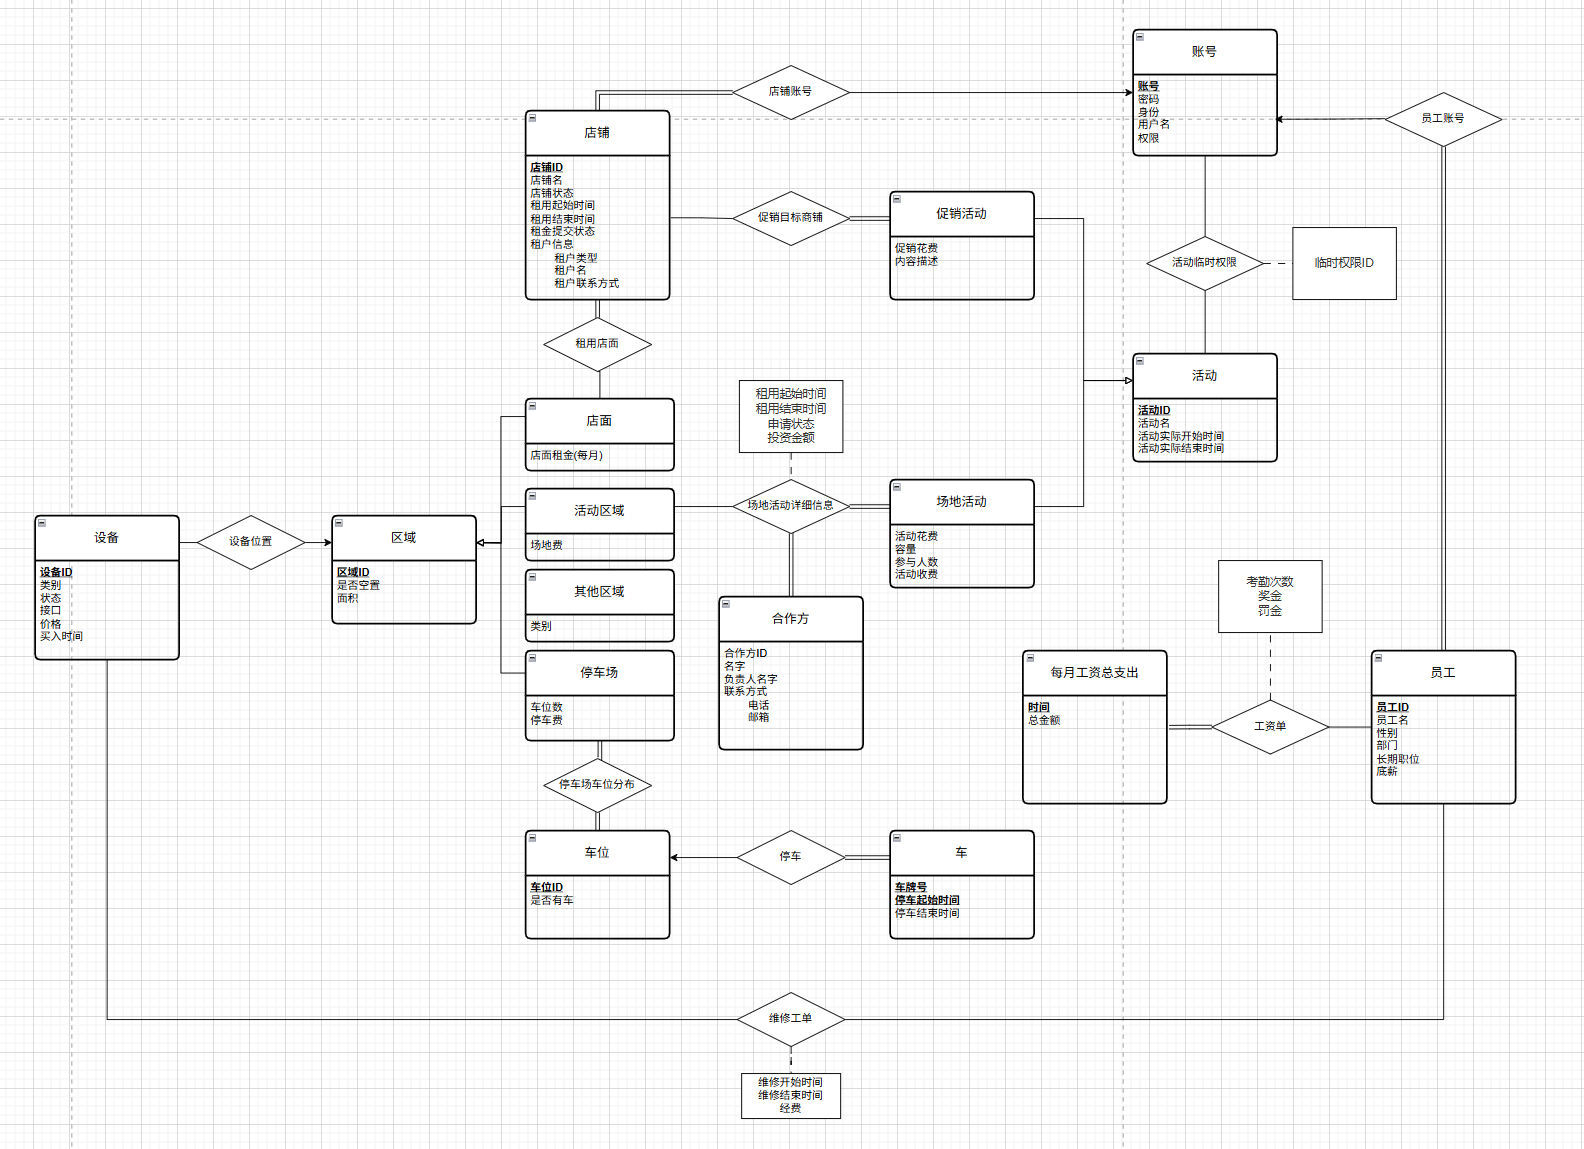
\includegraphics{image1.png}
\caption{总体E-R图}
\end{figure}

\hypertarget{ux6a21ux5757e-rux56fe}{%
\subsection{模块E-R图}\label{ux6a21ux5757e-rux56fe}}

\hypertarget{ux79dfux7528ux5e97ux9762e-rux56fe}{%
\subsubsection{租用店面E-R图}\label{ux79dfux7528ux5e97ux9762e-rux56fe}}

对于每个店铺,店铺需要依托于一个或多个实际的店面区域存在;但是对于每个店面,店面可以空置或者上面建设一个店铺。故该联系集中店铺和店面是一对多的关系,其中店铺为全参与。

\begin{figure}[htbp]
\centering
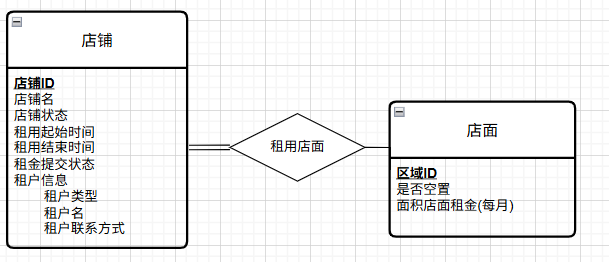
\includegraphics{image2.png}
\caption{租用店面E-R图}
\end{figure}

\hypertarget{ux505cux8f66e-rux56fe}{%
\subsubsection{停车E-R图}\label{ux505cux8f66e-rux56fe}}

对于每个车位,一个车位可以实时对应一辆或者不对应正在停的车;但是对于每一辆进入停车场被记录的车一定要有一个车位与其对应。故该联系集中车位和车是一对一关系,其中车是全参与。

\begin{figure}[htbp]
\centering
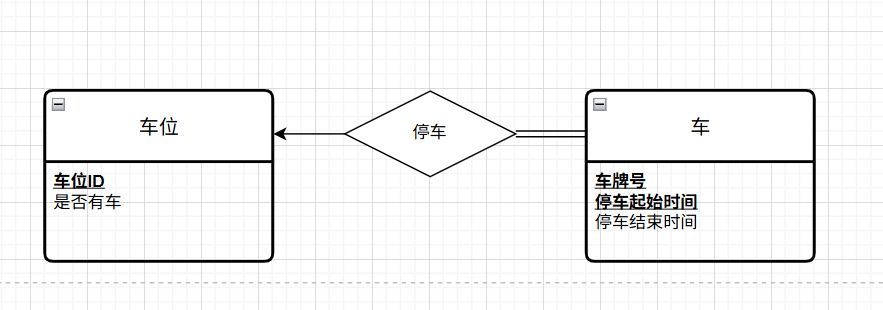
\includegraphics{image3.png}
\caption{停车E-R图}
\end{figure}

\hypertarget{ux505cux8f66ux573aux8f66ux4f4dux5206ux5e03e-rux56fe}{%
\subsubsection{停车场车位分布E-R图}\label{ux505cux8f66ux573aux8f66ux4f4dux5206ux5e03e-rux56fe}}

对于每个停车场区域内,一个停车场区域内可以包含多个车位,每个车位必须要依托于一个停车场区域存在并计算停车费用。故该联系集中车位和停车场是多对一的关系,二者均为全参与。

\begin{figure}[htbp]
\centering
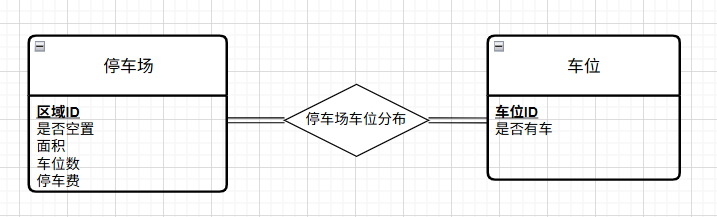
\includegraphics{image4.png}
\caption{停车场车位分布E-R图}
\end{figure}

\hypertarget{ux573aux5730ux6d3bux52a8ux8be6ux7ec6ux4fe1ux606fe-rux56fe}{%
\subsubsection{场地活动详细信息E-R图}\label{ux573aux5730ux6d3bux52a8ux8be6ux7ec6ux4fe1ux606fe-rux56fe}}

对于每个场地活动,一个活动需要关联一片或者多片活动区域,需要关联一个或多个合作方来进行投资或者参与。因此该三元联系集以活动为基础进行搭建,其中场地活动和合作方为全参与。

\begin{figure}[htbp]
\centering
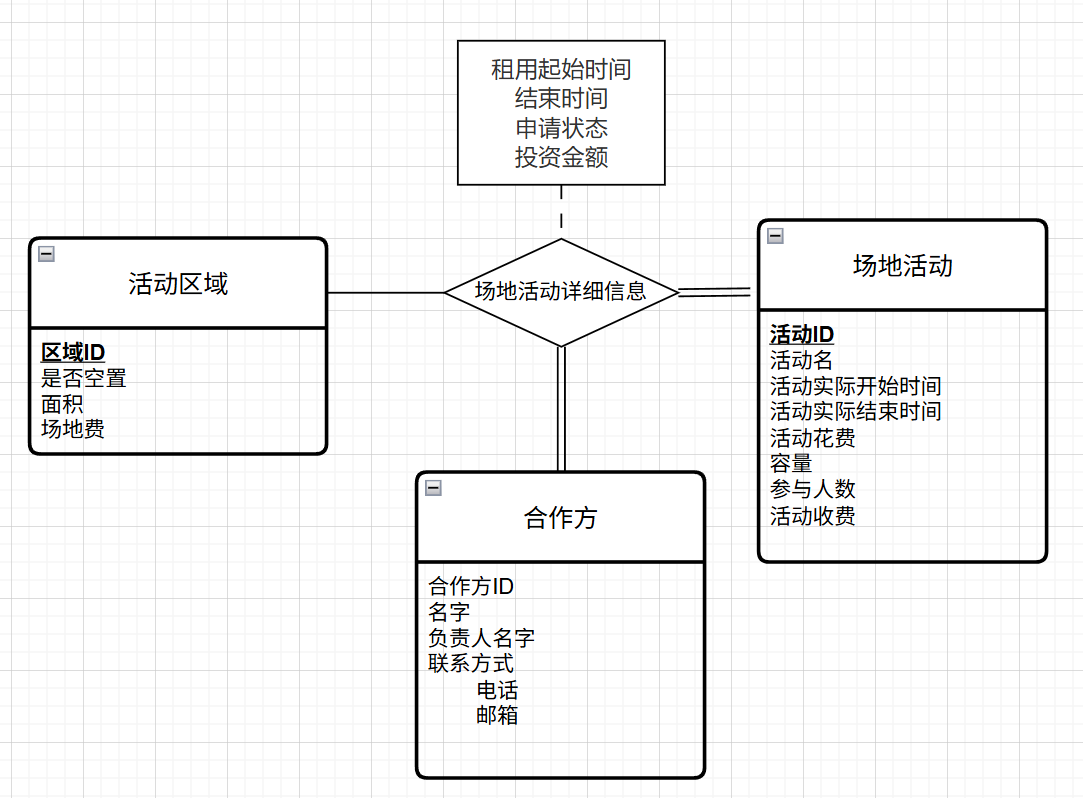
\includegraphics{image5.png}
\caption{场地活动详细信息E-R图}
\end{figure}

\hypertarget{ux4fc3ux9500ux76eeux6807ux5546ux94fae-rux56fe}{%
\subsubsection{促销目标商铺E-R图}\label{ux4fc3ux9500ux76eeux6807ux5546ux94fae-rux56fe}}

每个促销活动需要与特定店铺联系后才可应用,而每个店铺可以不和促销活动相关联或者和一到多个活动相关。因此该联系集中店铺和促销活动之间是多对多的关系,其中促销活动是全参与。

\begin{figure}[htbp]
\centering
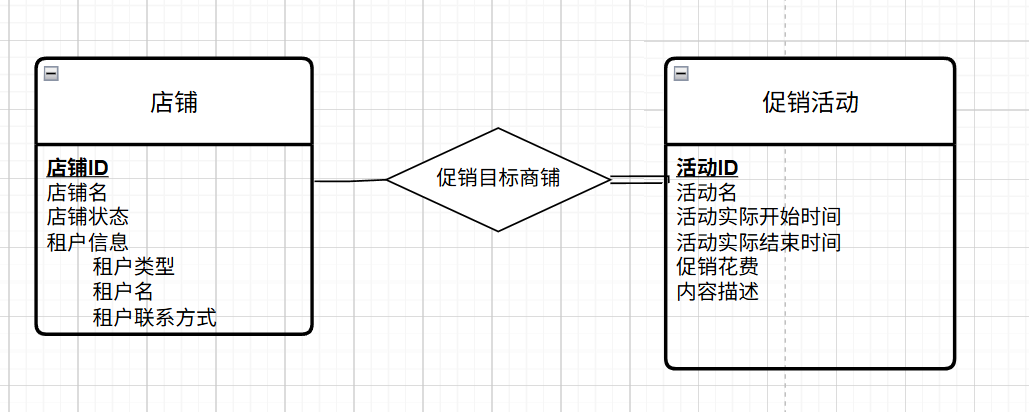
\includegraphics{image6.png}
\caption{促销目标商铺E-R图}
\end{figure}

\hypertarget{ux6d3bux52a8ux4e34ux65f6ux6743ux9650e-rux56fe}{%
\subsubsection{活动临时权限E-R图}\label{ux6d3bux52a8ux4e34ux65f6ux6743ux9650e-rux56fe}}

每个账号可以在后端获取一个具体的权限,依靠该权限可以查阅有关数据。但是对于某个员工或者店铺的账号临时承办对接某特殊活动的情况可能会需要给临时权限。因此在该联系集中一个活动需要多个账号参与,一个账号可以同时参与多个活动的进行。因此该联系集中账号和属性均为多对多关系。其属性为活动ID(主码)、账号(主码),有关联属性临时权限标识符,通过该属性可以从后端取得相应权限,在该联系结束时该权限也一并消失。

\begin{figure}[htbp]
\centering
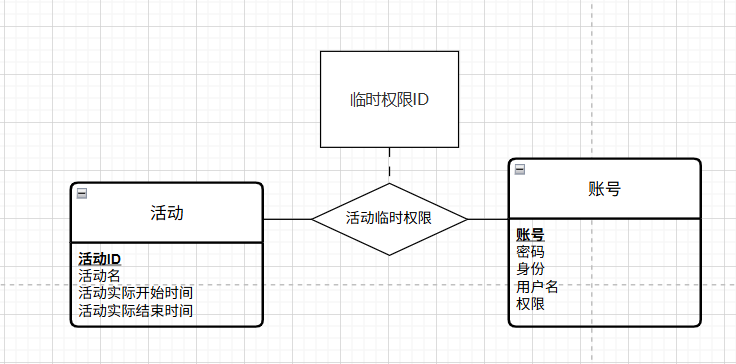
\includegraphics{image7.png}
\caption{活动临时权限模块E-R图}
\end{figure}

\hypertarget{ux8bbeux5907ux4f4dux7f6ee-rux56fe}{%
\subsubsection{设备位置E-R图}\label{ux8bbeux5907ux4f4dux7f6ee-rux56fe}}

该联系集用于标识设备所处的具体位置。每个设备必须要有一个对应的区域,每个区域可以对应一个或多个设备或是不对应任何设备。因此该联系集中设备和区域为多对一联系,其中设备为全参与。

\begin{figure}[htbp]
\centering
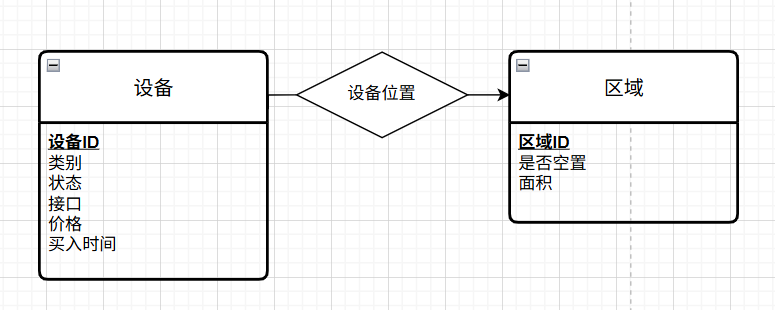
\includegraphics{image8.png}
\caption{设备位置E-R图}
\end{figure}

\hypertarget{ux7ef4ux4feeux5de5ux5355e-rux56fe}{%
\subsubsection{维修工单E-R图}\label{ux7ef4ux4feeux5de5ux5355e-rux56fe}}

该联系集用于联系损坏设备和修理员工。一个损坏设备可以给多个员工维修,一个员工也可以同时负责多台设备。因此该联系集中损坏设备和修理员工为多对多联系。

\begin{figure}[htbp]
\centering
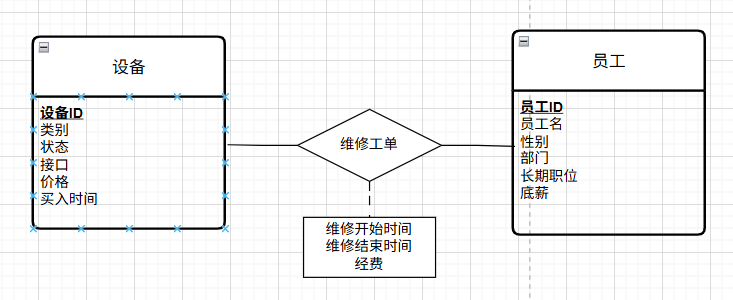
\includegraphics{image9.png}
\caption{维修工单E-R图}
\end{figure}

\hypertarget{ux5458ux5de5ux8d26ux53f7e-rux56fe}{%
\subsubsection{员工账号E-R图}\label{ux5458ux5de5ux8d26ux53f7e-rux56fe}}

该联系集用于联系员工实体和其拥有的员工账号。一个员工只能有一个对应的员工账号。因此该联系集中员工和账号为一对一联系。属性有账号(主码)、员工ID(主码)。

\begin{figure}[htbp]
\centering
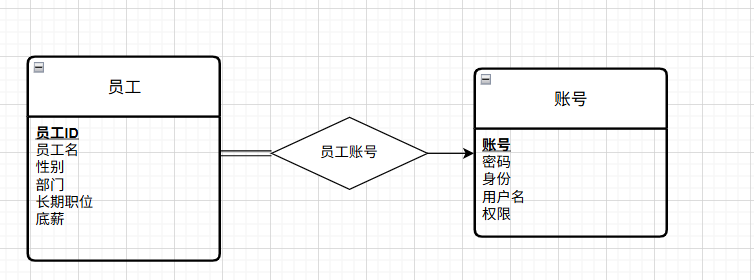
\includegraphics{image10.png}
\caption{员工账号E-R图}
\end{figure}

\hypertarget{ux5e97ux94faux8d26ux53f7e-rux56fe}{%
\subsubsection{店铺账号E-R图}\label{ux5e97ux94faux8d26ux53f7e-rux56fe}}

该联系集用于联系店铺实体和其拥有的店铺账号。一个店铺只能有一个对应的店铺账号。因此该联系集中店铺和账号为一对一联系。属性有账号(主码)、店铺ID(主码)。

\begin{figure}[htbp]
\centering
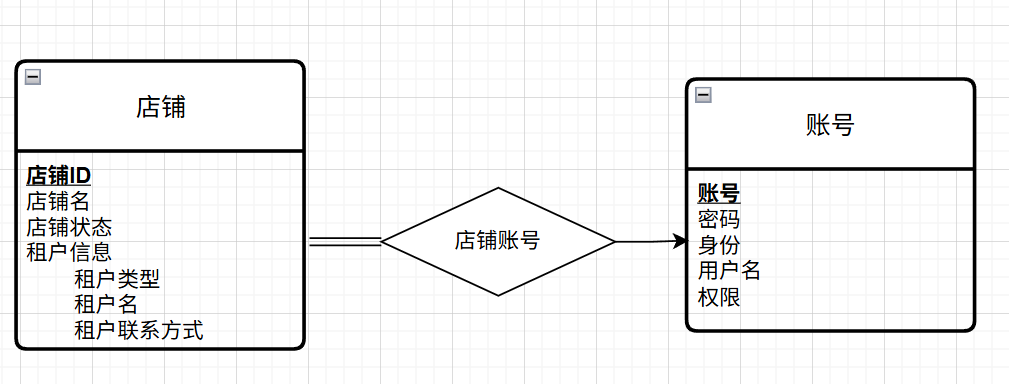
\includegraphics{image11.png}
\caption{店铺账号E-R图}
\end{figure}

\hypertarget{ux5de5ux8d44ux5355e-rux56fe}{%
\subsubsection{工资单E-R图}\label{ux5de5ux8d44ux5355e-rux56fe}}

该联系集用于联系员工实体和每月的工资发放情况,一个员工对应多个每月工资总支出,一个每月工资总支出又要对应多个员工。故该联系集为多对多联系。属性有员工ID(主码)、时间(主码),关联属性有考勤次数,跟月份对应记录其考勤状况,奖金、罚金用于综合计算薪水。

\begin{figure}[htbp]
\centering
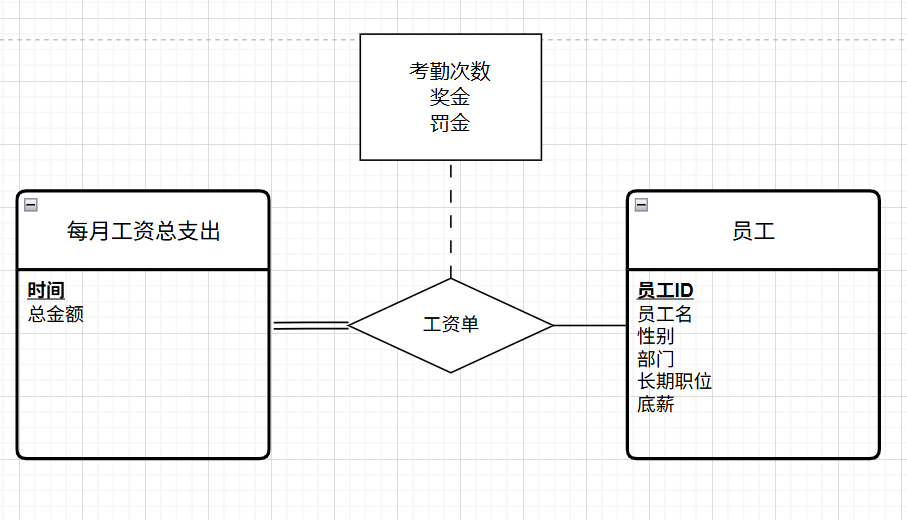
\includegraphics{image12.png}
\caption{工资单E-R图}
\end{figure}

\hypertarget{ux533aux57dfux7684ux7279ux5316e-rux56fe}{%
\subsubsection{区域的特化E-R图}\label{ux533aux57dfux7684ux7279ux5316e-rux56fe}}

对区域仅保留ID等基本属性,其余涉及到具体开店、举办活动、停车的部分分类特化给店面、活动区域、停车场三个部分执行。

\begin{figure}[htbp]
\centering
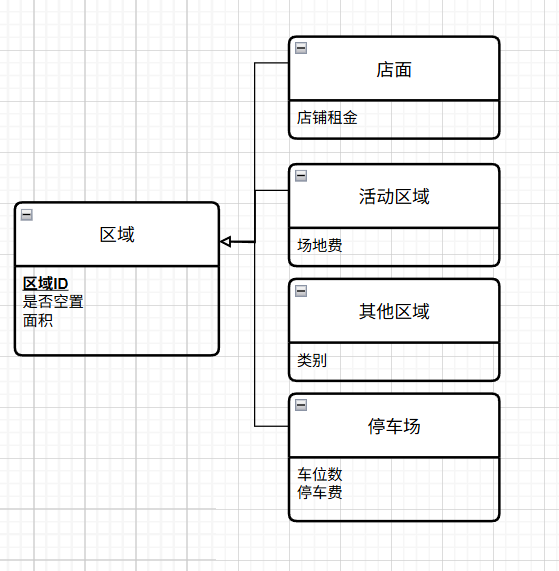
\includegraphics{image13.png}
\caption{区域的特化E-R图}
\end{figure}

\hypertarget{ux6d3bux52a8ux7684ux7279ux5316e-rux56fe}{%
\subsubsection{活动的特化E-R图}\label{ux6d3bux52a8ux7684ux7279ux5316e-rux56fe}}

活动仅保留基本信息,其余根据活动类型分类特化为促销活动和场地活动来和不同的实体集联系。

\begin{figure}[htbp]
\centering
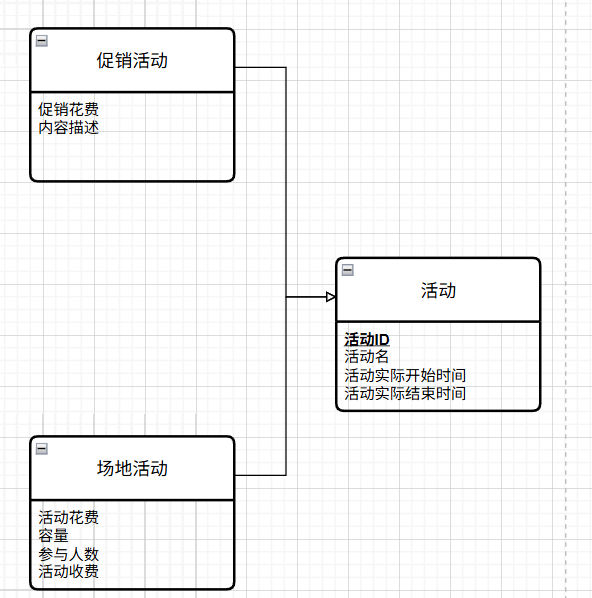
\includegraphics{image14.png}
\caption{活动的特化E-R图}
\end{figure}

\hypertarget{ux5173ux7cfbux6a21ux5f0f}{%
\subsection{关系模式}\label{ux5173ux7cfbux6a21ux5f0f}}

\hypertarget{ux5b9eux4f53ux96c6ux5173ux7cfbux6a21ux5f0f}{%
\subsubsection{实体集关系模式}\label{ux5b9eux4f53ux96c6ux5173ux7cfbux6a21ux5f0f}}

\begin{enumerate}
\def\labelenumi{\arabic{enumi}.}
\tightlist
\item
  店面(特化自区域)

  属性:区域ID(主键,外键引用区域), 出租情况, 店铺租金
\item
  店铺

  属性:店铺ID(主键), 店铺名称, 店铺状态(正常营业/打烊/歇业/翻新),
  租户类型(个人/企业连锁), 租户名, 租户联系方式
\item
  区域

  属性:区域ID(主键), 是否空置, 区域面积, 类别(区分店面/停车场/活动场地/其他区域)

  特化处理:

  其他区域(继承自区域):区域ID(主键,外键引用区域),
  类别(如卫生间、杂物间)
\item
  车位

  属性:车位ID(主键), 是否有车
\item
  车

  属性:车牌号(主键), 停车起始时间
\item
  停车场(特化自区域)

  属性:区域ID(主键,外键引用区域), 是否空置, 场地费
\item
  活动区域(特化自区域)

  属性:区域ID(主键,外键引用区域), 场地费, 容量, 是否空置
\item
  活动

  属性:活动ID(主键), 活动名, 活动开始时间, 活动结束时间

  特化处理:

  促销活动(继承自活动):活动ID(主键,外键引用活动), 促销花费, 内容描述

  场地活动(继承自活动):活动ID(主键,外键引用活动), '活动名', 参与人数,
  活动收费
\item
  员工

  属性:员工ID(主键), 员工名, 性别, 部门, 长期职位, 底薪, 本月出勤次数
\item
  合作方

  属性:合作方ID(主键), 名字, 负责人名, 联系方式 {电话, 邮箱}
\item
  设备

  属性:设备ID(主键), 类别, 状态, 接口, 价格, 买入时间
\item
  账号

  属性:账号(主键), 密码, 身份(商家/员工/游客/参演人员), 用户名
\item
  每月工资总支出

  属性:时间(主键),总金额
\end{enumerate}

\hypertarget{ux8054ux7cfbux96c6ux5173ux7cfbux6a21ux5f0f}{%
\subsubsection{联系集关系模式}\label{ux8054ux7cfbux96c6ux5173ux7cfbux6a21ux5f0f}}

\begin{enumerate}
\def\labelenumi{\arabic{enumi}.}
\tightlist
\item
  租用店面(店铺与店面)

  属性:店铺ID(外键引用店铺), 区域ID(外键引用店面), 租用起始时间, 持续时间,
  每月租金提交状态
\item
  停车(车与车位)

  属性:车牌号(外键引用车), 车位ID(外键引用车位)
\item
  停车场车位分布(车位与停车场)

  属性:车位ID(外键引用车位), 区域ID(外键引用停车场)
\item
  场地活动详细(活动场地、场地活动、合作方)

  属性:活动ID(外键引用场地活动), 区域ID(外键引用活动场地),
  合作方ID(外键引用合作方), 租用起始时间, 租用结束时间, 申请状态, 投资金额
\item
  促销目标商铺(促销活动与店铺)

  属性:活动ID(外键引用促销活动), 店铺ID(外键引用店铺)
\item
  活动临时权限(账号与活动)

  属性:账号(外键引用账号), 活动ID(外键引用活动), 临时权限ID
\item
  设备位置(设备与区域)

  属性:设备ID(外键引用设备), 区域ID(外键引用区域)
\item
  维修工单(设备与员工)

  属性:设备ID(外键引用设备), 员工ID(外键引用员工), 维修开始时间,维修结束时间,
  维修花费
\item
  商家账号(账号与店铺)

  属性:账号(外键引用账号), 店铺ID(外键引用店铺)
\item
  员工账号(账号与员工)

  属性:账号(外键引用账号), 员工ID(外键引用员工)
\item
  游客或参演人员账号(账号与场地活动)

  属性:账号(外键引用账号), 活动ID(外键引用场地活动)
\item
  工资单(员工与每月工资总支出)

  属性:员工ID(外键引用员工),时间(外键引用每月工资总支出),考勤次数,奖金,罚金
\end{enumerate}

\hypertarget{ux8868ux7684ux8bbeux8ba1}{%
\subsection{表的设计}\label{ux8868ux7684ux8bbeux8ba1}}

\hypertarget{ux5b9eux4f53ux8868}{%
\subsubsection{实体表}\label{ux5b9eux4f53ux8868}}

\begin{longtable}[]{@{}lllll@{}}
\caption{区域表}\\
\toprule
字段名 & 数据类型 & 长度 & 说明 & 备注 \\
\midrule
\endfirsthead
\toprule
字段名 & 数据类型 & 长度 & 说明 & 备注 \\
\midrule
\endhead
区域ID & INT & 11 & 唯一标识符 & PK \\
是否空置 & TINYINT & 1 & 0-否,1-是 & \\
区域面积 & DECIMAL & (10,2) & 单位:平方米 & \\
\bottomrule
\end{longtable}

\begin{longtable}[]{@{}lllll@{}}
\caption{店面表(特化自区域)}\\
\toprule
字段名 & 数据类型 & 长度 & 说明 & 备注 \\
\midrule
\endfirsthead
\toprule
字段名 & 数据类型 & 长度 & 说明 & 备注 \\
\midrule
\endhead
区域ID & INT & 11 & 唯一标识符 & PK,FK引用区域表 \\
出租情况 & VARCHAR & 20 & 出租状态 & \\
店铺租金 & DECIMAL & (10,2) & 每月租金 & \\
\bottomrule
\end{longtable}

\begin{longtable}[]{@{}lllll@{}}
\caption{其他区域表(特化自区域)}\\
\toprule
字段名 & 数据类型 & 长度 & 说明 & 备注 \\
\midrule
\endfirsthead
\toprule
字段名 & 数据类型 & 长度 & 说明 & 备注 \\
\midrule
\endhead
区域ID & INT & 11 & 唯一标识符 & PK,FK引用区域表 \\
类别 & VARCHAR & 20 & 区域子类型 & 如卫生间,杂物间 \\
\bottomrule
\end{longtable}

\begin{longtable}[]{@{}lllll@{}}
\caption{停车场表(特化自区域)}\\
\toprule
字段名 & 数据类型 & 长度 & 说明 & 备注 \\
\midrule
\endfirsthead
\toprule
字段名 & 数据类型 & 长度 & 说明 & 备注 \\
\midrule
\endhead
区域ID & INT & 11 & 唯一标识符 & PK,FK引用区域表 \\
场地费 & DECIMAL & (10,2) & 单位:元/小时 & \\
\bottomrule
\end{longtable}

\begin{longtable}[]{@{}lllll@{}}
\caption{活动区域表(特化自区域)}\\
\toprule
字段名 & 数据类型 & 长度 & 说明 & 备注 \\
\midrule
\endfirsthead
\toprule
字段名 & 数据类型 & 长度 & 说明 & 备注 \\
\midrule
\endhead
区域ID & INT & 11 & 唯一标识符 & PK,FK引用区域表 \\
场地费 & DECIMAL & (10,2) & 单位:元/次 & \\
容量 & INT & 11 & 最大容纳人数 & \\
\bottomrule
\end{longtable}

\begin{longtable}[]{@{}lllll@{}}
\caption{店铺表}\\
\toprule
字段名 & 数据类型 & 长度 & 说明 & 备注 \\
\midrule
\endfirsthead
\toprule
字段名 & 数据类型 & 长度 & 说明 & 备注 \\
\midrule
\endhead
店铺ID & INT & 11 & 唯一标识符 & PK \\
店铺名称 & VARCHAR & 50 & 店铺名称 & \\
店铺状态 & VARCHAR & 20 & 营业状态 & 正常营业/打烊/歇业/翻新 \\
租户类型 & VARCHAR & 20 & 租户类型 & 个人/企业连锁 \\
租户名 & VARCHAR & 50 & 租户名称 & \\
租户联系方式 & VARCHAR & 100 & 联系方式 & 可存储电话或邮箱 \\
租用起始时间 & DATE &  & 租用开始计时 & \\
租用结束时间 & DATE &  & 租用结束计时 & \\
\bottomrule
\end{longtable}

\begin{longtable}[]{@{}lllll@{}}
\caption{车位表}\\
\toprule
字段名 & 数据类型 & 长度 & 说明 & 备注 \\
\midrule
\endfirsthead
\toprule
字段名 & 数据类型 & 长度 & 说明 & 备注 \\
\midrule
\endhead
车位ID & INT & 11 & 唯一标识符 & PK \\
是否有车 & TYNYINT & 1 & 0-否,1-是 & \\
\bottomrule
\end{longtable}

\begin{longtable}[]{@{}lllll@{}}
\caption{车表}\\
\toprule
字段名 & 数据类型 & 长度 & 说明 & 备注 \\
\midrule
\endfirsthead
\toprule
字段名 & 数据类型 & 长度 & 说明 & 备注 \\
\midrule
\endhead
车牌号 & VARCHAR & 20 & 车牌号 & PK-1 \\
停车起始时间 & DATE &  & 停车时间 & PK-2 \\
停车结束时间 & DATE &  & 停车结束的时间 & \\
\bottomrule
\end{longtable}

\begin{longtable}[]{@{}lllll@{}}
\caption{活动表}\\
\toprule
字段名 & 数据类型 & 长度 & 说明 & 备注 \\
\midrule
\endfirsthead
\toprule
字段名 & 数据类型 & 长度 & 说明 & 备注 \\
\midrule
\endhead
活动ID & INT & 11 & 唯一标识符 & PK \\
活动名 & VARCHAR & 50 & 活动名称 & \\
活动开始时间 & DATETIME &  & 开始时间 & \\
活动结束时间 & DATETIME &  & 结束时间 & \\
\bottomrule
\end{longtable}

\begin{longtable}[]{@{}lllll@{}}
\caption{促销活动表(特化自活动)}\\
\toprule
字段名 & 数据类型 & 长度 & 说明 & 备注 \\
\midrule
\endfirsthead
\toprule
字段名 & 数据类型 & 长度 & 说明 & 备注 \\
\midrule
\endhead
活动ID & INT & 11 & 唯一标识符 & PK,FK引用活动表 \\
促销花费 & DECIMAL & (10,2) & 总花费 & \\
内容描述 & VARCHAR & 1000 & 活动内容 & \\
\bottomrule
\end{longtable}

\begin{longtable}[]{@{}lllll@{}}
\caption{场地活动表(特化自活动)}\\
\toprule
字段名 & 数据类型 & 长度 & 说明 & 备注 \\
\midrule
\endfirsthead
\toprule
字段名 & 数据类型 & 长度 & 说明 & 备注 \\
\midrule
\endhead
活动ID & INT & 11 & 唯一标识符 & PK,FK引用活动表 \\
参与人数 & INT & 11 & 实际参与人数 & \\
活动收费 & DECIMAL & (10,2) & 单位:元/人 & \\
容量 & INT & 11 & 场地最大容纳人数 & \\
活动花费 & DEMICAL & (10,2) & 单位:元 & \\
\bottomrule
\end{longtable}

\begin{longtable}[]{@{}lllll@{}}
\caption{员工表}\\
\toprule
字段名 & 数据类型 & 长度 & 说明 & 备注 \\
\midrule
\endfirsthead
\toprule
字段名 & 数据类型 & 长度 & 说明 & 备注 \\
\midrule
\endhead
员工ID & INT & 11 & 唯一标识符 & PK \\
员工名 & VARCHAR & 50 & 员工姓名 & \\
性别 & VARCHAR & 10 & 性别 & \\
部门 & VARCHAR & 50 & 所属部门 & \\
长期职位 & VARCHAR & 50 & 职位名称 & \\
底薪 & DECIMAL & (10,2) & 月薪 & \\
\bottomrule
\end{longtable}

\begin{longtable}[]{@{}lllll@{}}
\caption{合作方表}\\
\toprule
字段名 & 数据类型 & 长度 & 说明 & 备注 \\
\midrule
\endfirsthead
\toprule
字段名 & 数据类型 & 长度 & 说明 & 备注 \\
\midrule
\endhead
合作方ID & INT & 11 & 唯一标识符 & PK \\
名字 & VARCHAR & 50 & 合作方名称 & \\
负责人名 & VARCHAR & 50 &  & \\
电话 & VARCHAR & 20 & 联系方式 & \\
邮箱 & VARCHAR & 50 & 联系方式 & \\
\bottomrule
\end{longtable}

\begin{longtable}[]{@{}lllll@{}}
\caption{设备表}\\
\toprule
字段名 & 数据类型 & 长度 & 说明 & 备注 \\
\midrule
\endfirsthead
\toprule
字段名 & 数据类型 & 长度 & 说明 & 备注 \\
\midrule
\endhead
设备ID & INT & 11 & 唯一标识符 & PK \\
类别 & VARCHAR & 50 & 设备类型 & 如空调、摄像头 \\
状态 & VARCHAR & 20 & 设备状态 & 正常/故障/维修中 \\
接口 & VARCHAR & 50 & 接口类型 & \\
价格 & DECIMAL & (10,2) & 购买价格 & \\
买入时间 & DATE &  & 购买日期 & \\
\bottomrule
\end{longtable}

\begin{longtable}[]{@{}lllll@{}}
\caption{账号表}\\
\toprule
字段名 & 数据类型 & 长度 & 说明 & 备注 \\
\midrule
\endfirsthead
\toprule
字段名 & 数据类型 & 长度 & 说明 & 备注 \\
\midrule
\endhead
账号 & VARCHAR & 50 & 唯一标识符 & PK \\
密码 & VARCHAR & 50 & 登录密码 & 加密存储 \\
身份 & VARCHAR & 20 & 用户身份 & 商家/员工 \\
用户名 & VARCHAR & 50 & 显示名称 & \\
权限 & INT & 11 & 以编码的形式进行权限分配 & \\
\bottomrule
\end{longtable}

\begin{longtable}[]{@{}lllll@{}}
\caption{每月工资总支出}\\
\toprule
字段名 & 数据类型 & 长度 & 说明 & 备注 \\
\midrule
\endfirsthead
\toprule
字段名 & 数据类型 & 长度 & 说明 & 备注 \\
\midrule
\endhead
时间 & DATETIME &  &  & PK \\
总金额 & DECIMAL & (10,2) & 每月给员工支出的总工资金额 & \\
\bottomrule
\end{longtable}

\hypertarget{ux8054ux7cfbux8868}{%
\subsubsection{联系表}\label{ux8054ux7cfbux8868}}

\begin{longtable}[]{@{}lllll@{}}
\caption{租用店面表}\\
\toprule
字段名 & 数据类型 & 长度 & 说明 & 备注 \\
\midrule
\endfirsthead
\toprule
字段名 & 数据类型 & 长度 & 说明 & 备注 \\
\midrule
\endhead
店铺ID & INT & 11 & 店铺标识符 & FK引用店铺表 \\
区域ID & INT & 11 & 店面标识符 & FK引用店铺表 \\
\bottomrule
\end{longtable}

\begin{longtable}[]{@{}lllll@{}}
\caption{停车表}\\
\toprule
字段名 & 数据类型 & 长度 & 说明 & 备注 \\
\midrule
\endfirsthead
\toprule
字段名 & 数据类型 & 长度 & 说明 & 备注 \\
\midrule
\endhead
车牌号 & VARCHAR & 20 & 车辆标识符 & 外键引用车表 \\
车位ID & INT & 11 & 车位标识符 & 外键引用车位表 \\
\bottomrule
\end{longtable}

\begin{longtable}[]{@{}lllll@{}}
\caption{停车场车位分布表}\\
\toprule
字段名 & 数据类型 & 长度 & 说明 & 备注 \\
\midrule
\endfirsthead
\toprule
字段名 & 数据类型 & 长度 & 说明 & 备注 \\
\midrule
\endhead
区域ID & INT & 11 & 停车场标识符 & 外键引用停车场表 \\
车位ID & INT & 11 & 车位标识符 & 外键引用车位表 \\
\bottomrule
\end{longtable}

\begin{longtable}[]{@{}lllll@{}}
\caption{场地活动详细表}\\
\toprule
字段名 & 数据类型 & 长度 & 说明 & 备注 \\
\midrule
\endfirsthead
\toprule
字段名 & 数据类型 & 长度 & 说明 & 备注 \\
\midrule
\endhead
活动ID & INT & 11 & 活动标识符 & FK引用场地活动表 \\
区域ID & INT & 11 & 活动场地标识符 & FK引用活动区域表 \\
合作方ID & INT & 11 & 合作方标识符 & FK引用合作方表 \\
租用起始时间 & DATE &  & 场地租用开始时间 & \\
租用结束时间 & DATE &  & 场地租用结束时间 & \\
申请状态 & VARCHAR & 20 & 活动申请状态 & 如"待审批""已通过" \\
投资金额 & DECIMAL & (10,2) & 合作方投资金额 & \\
\bottomrule
\end{longtable}

\begin{longtable}[]{@{}lllll@{}}
\caption{促销目标商铺表}\\
\toprule
字段名 & 数据类型 & 长度 & 说明 & 备注 \\
\midrule
\endfirsthead
\toprule
字段名 & 数据类型 & 长度 & 说明 & 备注 \\
\midrule
\endhead
活动ID & INT & 11 & 促销活动标识符 & FK引用促销活动表 \\
店铺ID & INT & 11 & 参与店铺标识符 & FK引用店铺表 \\
\bottomrule
\end{longtable}

\begin{longtable}[]{@{}lllll@{}}
\caption{活动临时权限表}\\
\toprule
字段名 & 数据类型 & 长度 & 说明 & 备注 \\
\midrule
\endfirsthead
\toprule
字段名 & 数据类型 & 长度 & 说明 & 备注 \\
\midrule
\endhead
账号 & VARCHAR & 50 &  & FK引用账号表 \\
活动ID & INT & 11 &  & FK引用活动表 \\
临时权限 & INT & 11 &  & 和权限一样,以编码形式分配权限 \\
权限内容 & VARCHAR & 100 & 权限描述 & 如"场地管理""设备操作" \\
\bottomrule
\end{longtable}

\begin{longtable}[]{@{}lllll@{}}
\caption{设备位置表}\\
\toprule
字段名 & 数据类型 & 长度 & 说明 & 备注 \\
\midrule
\endfirsthead
\toprule
字段名 & 数据类型 & 长度 & 说明 & 备注 \\
\midrule
\endhead
设备ID & INT & 11 & 设备标识符 & FK引用设备表 \\
区域ID & INT & 11 & 区域标识符 & FK引用区域表 \\
\bottomrule
\end{longtable}

\begin{longtable}[]{@{}lllll@{}}
\caption{维修工单表}\\
\toprule
字段名 & 数据类型 & 长度 & 说明 & 备注 \\
\midrule
\endfirsthead
\toprule
字段名 & 数据类型 & 长度 & 说明 & 备注 \\
\midrule
\endhead
设备ID & INT & 11 & 设备标识符 & FK引用设备表 \\
员工ID & INT & 11 & 维修员工标识符 & FK引用员工表 \\
报修开始时间 & DATE &  & 修理开始时间 & \\
维修结束时间 & DATE &  & 修理结束时间 & \\
维修花费 & DECIMAL & (10,2) & 维修费用 & \\
\bottomrule
\end{longtable}

\begin{longtable}[]{@{}lllll@{}}
\caption{商家账号表}\\
\toprule
字段名 & 数据类型 & 长度 & 说明 & 备注 \\
\midrule
\endfirsthead
\toprule
字段名 & 数据类型 & 长度 & 说明 & 备注 \\
\midrule
\endhead
账号 & VARCHAR & 50 & 账号标识符 & FK引用账号表 \\
店铺ID & INT & 11 & 店铺标识符 & FK引用店铺表 \\
\bottomrule
\end{longtable}

\begin{longtable}[]{@{}lllll@{}}
\caption{员工账号表}\\
\toprule
字段名 & 数据类型 & 长度 & 说明 & 备注 \\
\midrule
\endfirsthead
\toprule
字段名 & 数据类型 & 长度 & 说明 & 备注 \\
\midrule
\endhead
账号 & VARCHAR & 50 & 账号标识符 & FK引用账号表 \\
员工ID & INT & 11 & 员工标识符 & FK引用员工表 \\
\bottomrule
\end{longtable}

\begin{longtable}[]{@{}lllll@{}}
\caption{工资单表}\\
\toprule
字段名 & 数据类型 & 长度 & 说明 & 备注 \\
\midrule
\endfirsthead
\toprule
字段名 & 数据类型 & 长度 & 说明 & 备注 \\
\midrule
\endhead
员工ID & INT & 11 & 账号标识符 & PK,FK引用员工表 \\
时间 & DATETIME &  &  & PK,FK引用每月工资总支出表 \\
考勤次数 & INT & 3 & 员工每月考勤次数 & \\
奖金 & DECIMAL & (10,2) &  & \\
罚金 & DECIMAL & (10,2) &  & \\
\bottomrule
\end{longtable}

\hypertarget{ux6570ux636eux5e93ux5173ux7cfbux56fe}{%
\subsection{数据库关系图}\label{ux6570ux636eux5e93ux5173ux7cfbux56fe}}

\begin{figure}[htbp]
\centering
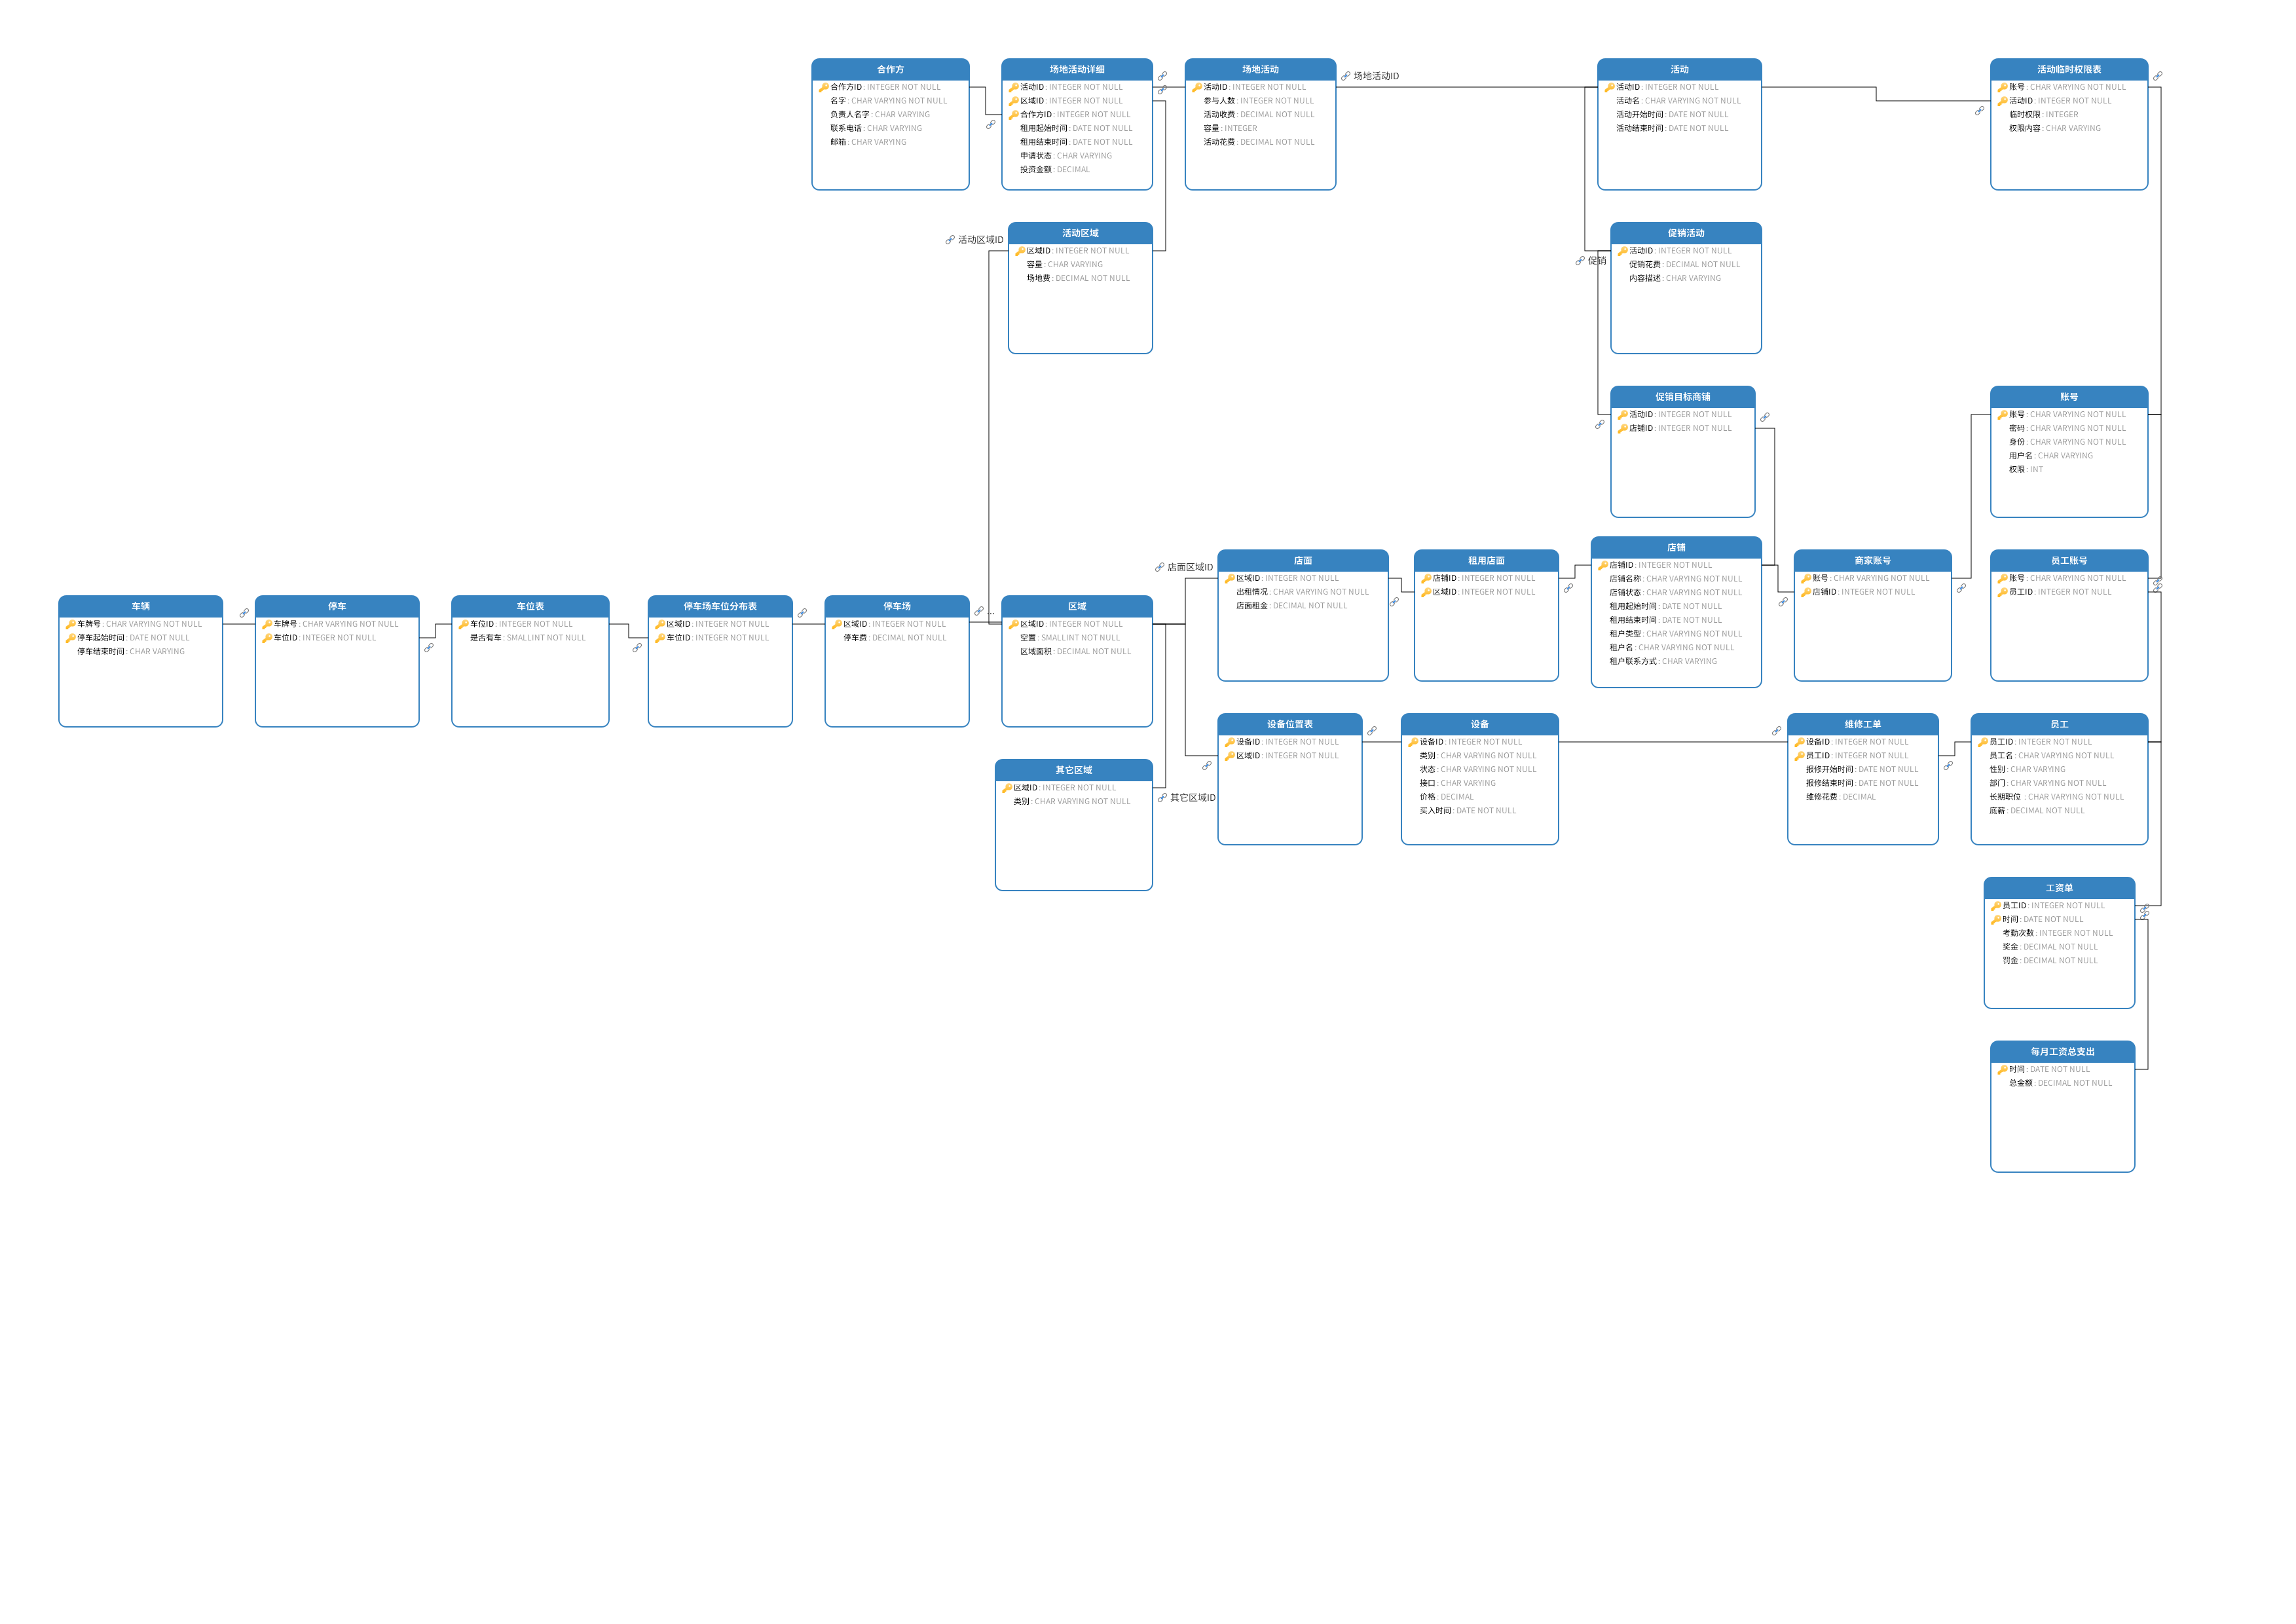
\includegraphics{image15.png}
\caption{数据库关系图}
\end{figure}

\end{document}